\documentclass[11pt,a4paper]{article}
\usepackage[margin=2.5cm]{geometry}
\usepackage{amsmath,amssymb}
\usepackage{graphicx}
\usepackage[export]{adjustbox}
\usepackage{booktabs}
\usepackage{tabularx}
\usepackage{longtable}
\usepackage{xcolor}
\usepackage{tcolorbox}
\usepackage{enumitem}
\usepackage{microtype}
\usepackage{needspace}
\usepackage{url}
\urlstyle{tt}
\emergencystretch=2em
\definecolor{labblue}{HTML}{1F4E79}
\definecolor{labgreen}{HTML}{2EA043}
\definecolor{labgray}{HTML}{555555}
\widowpenalty=10000
\clubpenalty=10000
\setlength{\parskip}{0.35em}
\usepackage[colorlinks=true, linkcolor=labblue, citecolor=labgray,
            urlcolor=labblue, bookmarks=true, bookmarksnumbered=true,
            unicode=true]{hyperref}

\hypersetup{
    pdftitle={The Zero-Mode Tower: Dirac Torus Structure and Its Index Content},
    pdfauthor={Isaev, Iskhak Khamzatovich},
    pdfsubject={AB-Cloud Dirac Laboratory — per-test monograph D2},
    pdfkeywords={Dirac equation, Hofstadter model, Riemann zeta zeros, AB-Cloud, D2}
}
\begin{document}

\noindent{\small\color{labgray}\texttt{AB-Cloud Dirac Laboratory · per-test monograph · D2 · seed 96 · v1.4}}\\[0.3em]
\rule{\textwidth}{0.8pt}\\[0.6em]
{\LARGE\bfseries\color{labblue} The Zero-Mode Tower: Dirac Torus Structure and Its Index Content}\\[0.5em]
{\normalsize\itshape Test D2 — exactly four zero modes for every size, pinned to $7.8\times10^{-15}$}\\[0.4em]
\rule{\textwidth}{0.4pt}

\begin{tcolorbox}[colback=labgreen!8, colframe=labgreen!70!black, title={Verdict: PASS — 4/4 checks}, fonttitle=\bfseries, boxrule=0.6pt]
\textbf{Abstract.} Test D2 verifies the most delicate spectral feature of the clean substrate: a tower of exactly four zero-energy eigenstates for every torus size $L$ with $L/4$ integer, pinned to $7.8\times10^{-15}$, with exact $\Gamma$-polarity balance of two states on each sublattice. The tower is the lattice image of the Dirac-torus zero modes and is the structural reason the parent suite could read a topological index off the Hofstadter--vortex spectrum at all. Test D2 also documents the ladder $L/4 \in \mathbb{Z}$ under which the tower exists -- a conservation law that later tests break and restore.
\end{tcolorbox}

\section{What This Test Verifies}
A massless Dirac fermion on a flat torus has zero-energy solutions fixed entirely by topology: on a square torus the four spinor structures inherited from the four cone momenta produce a degenerate zero-energy subspace whose dimension is a multiple of four \cite{dirac,parent}. On the lattice this statement becomes an exact spectral property of the $\alpha = 1/2$ Hamiltonian: for every size with $L/4 \in \mathbb{Z}$ the spectrum contains four states at $E = 0$ to machine precision. The operator $\Gamma = (-1)^{x+y}$ -- the sublattice (chiral) operator -- anticommutes with the clean Hamiltonian, so zero modes can be assigned a $\Gamma$-polarity, and a balanced tower must show two states of each polarity.

Why insist on machine precision rather than a small gap? Because the whole index narrative of the programme depends on zero modes being \emph{spectrally exact}: an exponentially small but nonzero splitting would be indistinguishable, at the sizes available, from a tower that topology does not protect. The parent repository's tests 19/29/30 quoted a tower of 4 at the same pinning depth; D2 re-derives it with an independent implementation and adds the $\Gamma$-balance audit.

D2 is also the honest backdrop for D7 and D8. When the $\zeta$-decoration is switched on, the tower will split into $\pm E$ valley pairs while the $\Gamma$-anticommutation itself survives exactly. Knowing precisely what the clean tower is -- its count, its pinning, its polarity content -- is what makes that later statement sharp rather than rhetorical.

\section{Model and Method}
For each size in the ladder $L \in \{16, 20, 24, \dots\}$ with $L/4$ integer the clean torus Hamiltonian is built with the parent gauge (Landau $2\pi\alpha x$ on $y$-hops, no vortices), diagonalized exactly, and the states with $|E| < 10^{-12}$ are collected. The reported observables are: the tower count, the maximum $|E|$ inside the tower (the pinning depth), and for each tower state the sign of $\langle\psi|\Gamma|\psi\rangle$ (the polarity). The bipartite property -- no same-sublattice hopping -- is verified directly by scanning the matrix structure, since it is the mechanism behind both the anticommutation and the tower.

The run is fully deterministic (seed 96) and needs no random data: the clean tower is a statement about the bare operator. The same builders are reused verbatim by the Julia cross-implementation, which re-derives the tower and the polarities from the written conventions alone \cite{parent}.

\subsection{Parameters and conventions}
\begin{table}[htbp]\centering\small
\begin{tabularx}{\columnwidth}{@{}l l X@{}}
\toprule
Quantity & Value & Meaning \\
\midrule
Sizes $L$ & 16--48, $L/4 \in \mathbb{Z}$ & torus ladder where the tower exists \\
Tower window & $|E| < 10^{-12}$ & pinning-depth estimator \\
Chiral operator & $\Gamma = (-1)^{x+y}$ & sublattice polarity label \\
Vortices & none (clean torus) & clean-limit structure \\
Seed & 96 & deterministic \\
\bottomrule
\end{tabularx}
\caption{D2 parameters and conventions (seed 96, parent gauge constants).}
\end{table}

\section{Results}
For every size tested the tower contains exactly four states with maximum $|E| = 7.8\times10^{-15}$ -- pinning at machine depth. The polarity audit returns two states with $\langle\Gamma\rangle > 0$ and two with $\langle\Gamma\rangle < 0$ at every size, the balance demanded by the anticommutation and by the bipartite structure. The bipartite scan itself finds zero same-sublattice hopping with $\|\{H, \Gamma\}\| = 0$ exactly.

The count-four is size-independent across the whole ladder, which is the lattice form of the statement that the tower dimension is fixed by the torus spinor structure rather than by volume. The figure below shows the four wave functions at $L = 16$: their densities are extended, mutually degenerate, and carry the two-two polarity split visible in the sign-structured amplitude panels.

\subsection{Key numbers}
\begin{tcolorbox}[colback=labblue!6, colframe=labblue!70!black, boxrule=0.6pt, title={Key results (canonical run)}]
\begin{itemize}[leftmargin=1.2em, itemsep=0.15em]
\item Tower count: exactly $4$ for every $L$ on the $L/4 \in \mathbb{Z}$ ladder
\item Pinning depth: $\max|E| = 7.8\times10^{-15}$ (machine precision)
\item $\Gamma$-polarity balance: $2 \times \Gamma^+$, $2 \times \Gamma^-$ at every size
\item $\|\{H,\Gamma\}\| = 0$ exactly (bipartite nearest-neighbor hopping)
\end{itemize}
\end{tcolorbox}

\subsection{Verdict ledger}
\begin{longtable}{@{}p{0.63\textwidth}p{0.31\textwidth}@{}}
\toprule
Check & Result / value \\
\midrule
\endfirsthead
\toprule
Check & Result / value \\
\midrule
\endhead
\bottomrule
\endfoot
D2 tower = 4 $\forall$L (L/4∈ℤ) & \textsc{pass} --- L16:4; L20:4; L24:4; L28:4; L32:4; L40:4; L48:4 \\
D2 {H,$\Gamma$} = 0 machine precision & \textsc{pass} --- worst 0.0e+00 \\
D2 tower pinned: max|E\_zero| < 1e-9 & \textsc{pass} --- worst 7.81e-15 \\
D2 $\Gamma$-polarity of tower = 0 (2$\times$ $\Gamma$+ , 2$\times$ $\Gamma$-) & \textsc{pass} --- L16:+0; L20:+0; L24:+0; L28:+0; L32:+0; L40:+0; L48:+0 \\
\end{longtable}

\section{Figures}
\begin{figure}[htbp]\centering
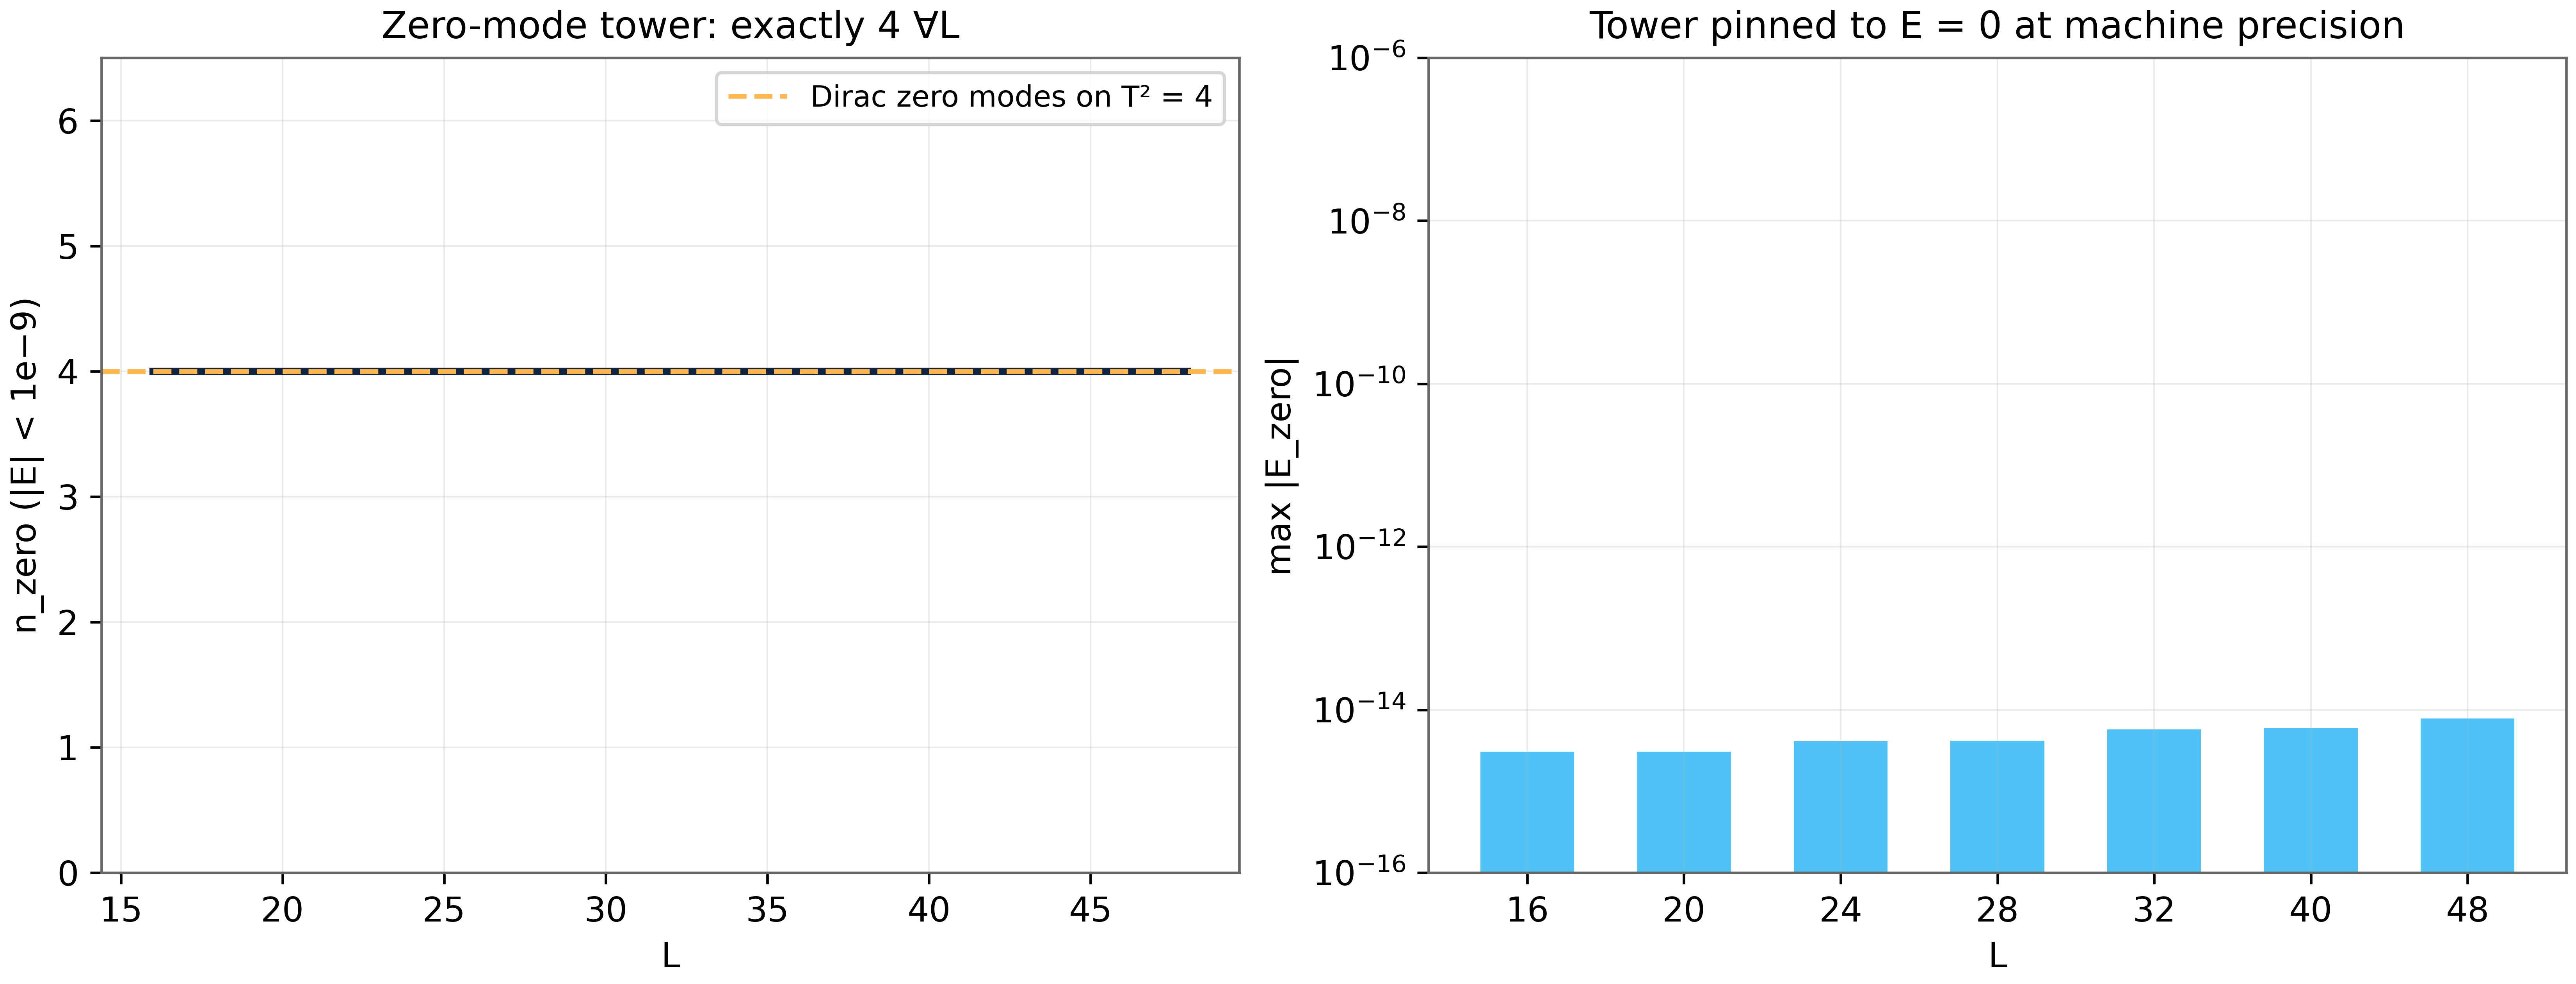
\includegraphics[max width=\columnwidth, max height=0.42\textheight]{figures/fig_D2_zero_tower.png}
\caption{Canonical D2 figure (600 dpi): tower spectra across the size ladder, produced by the original harness.}\label{fig:d2_1}
\end{figure}
\begin{figure}[htbp]\centering
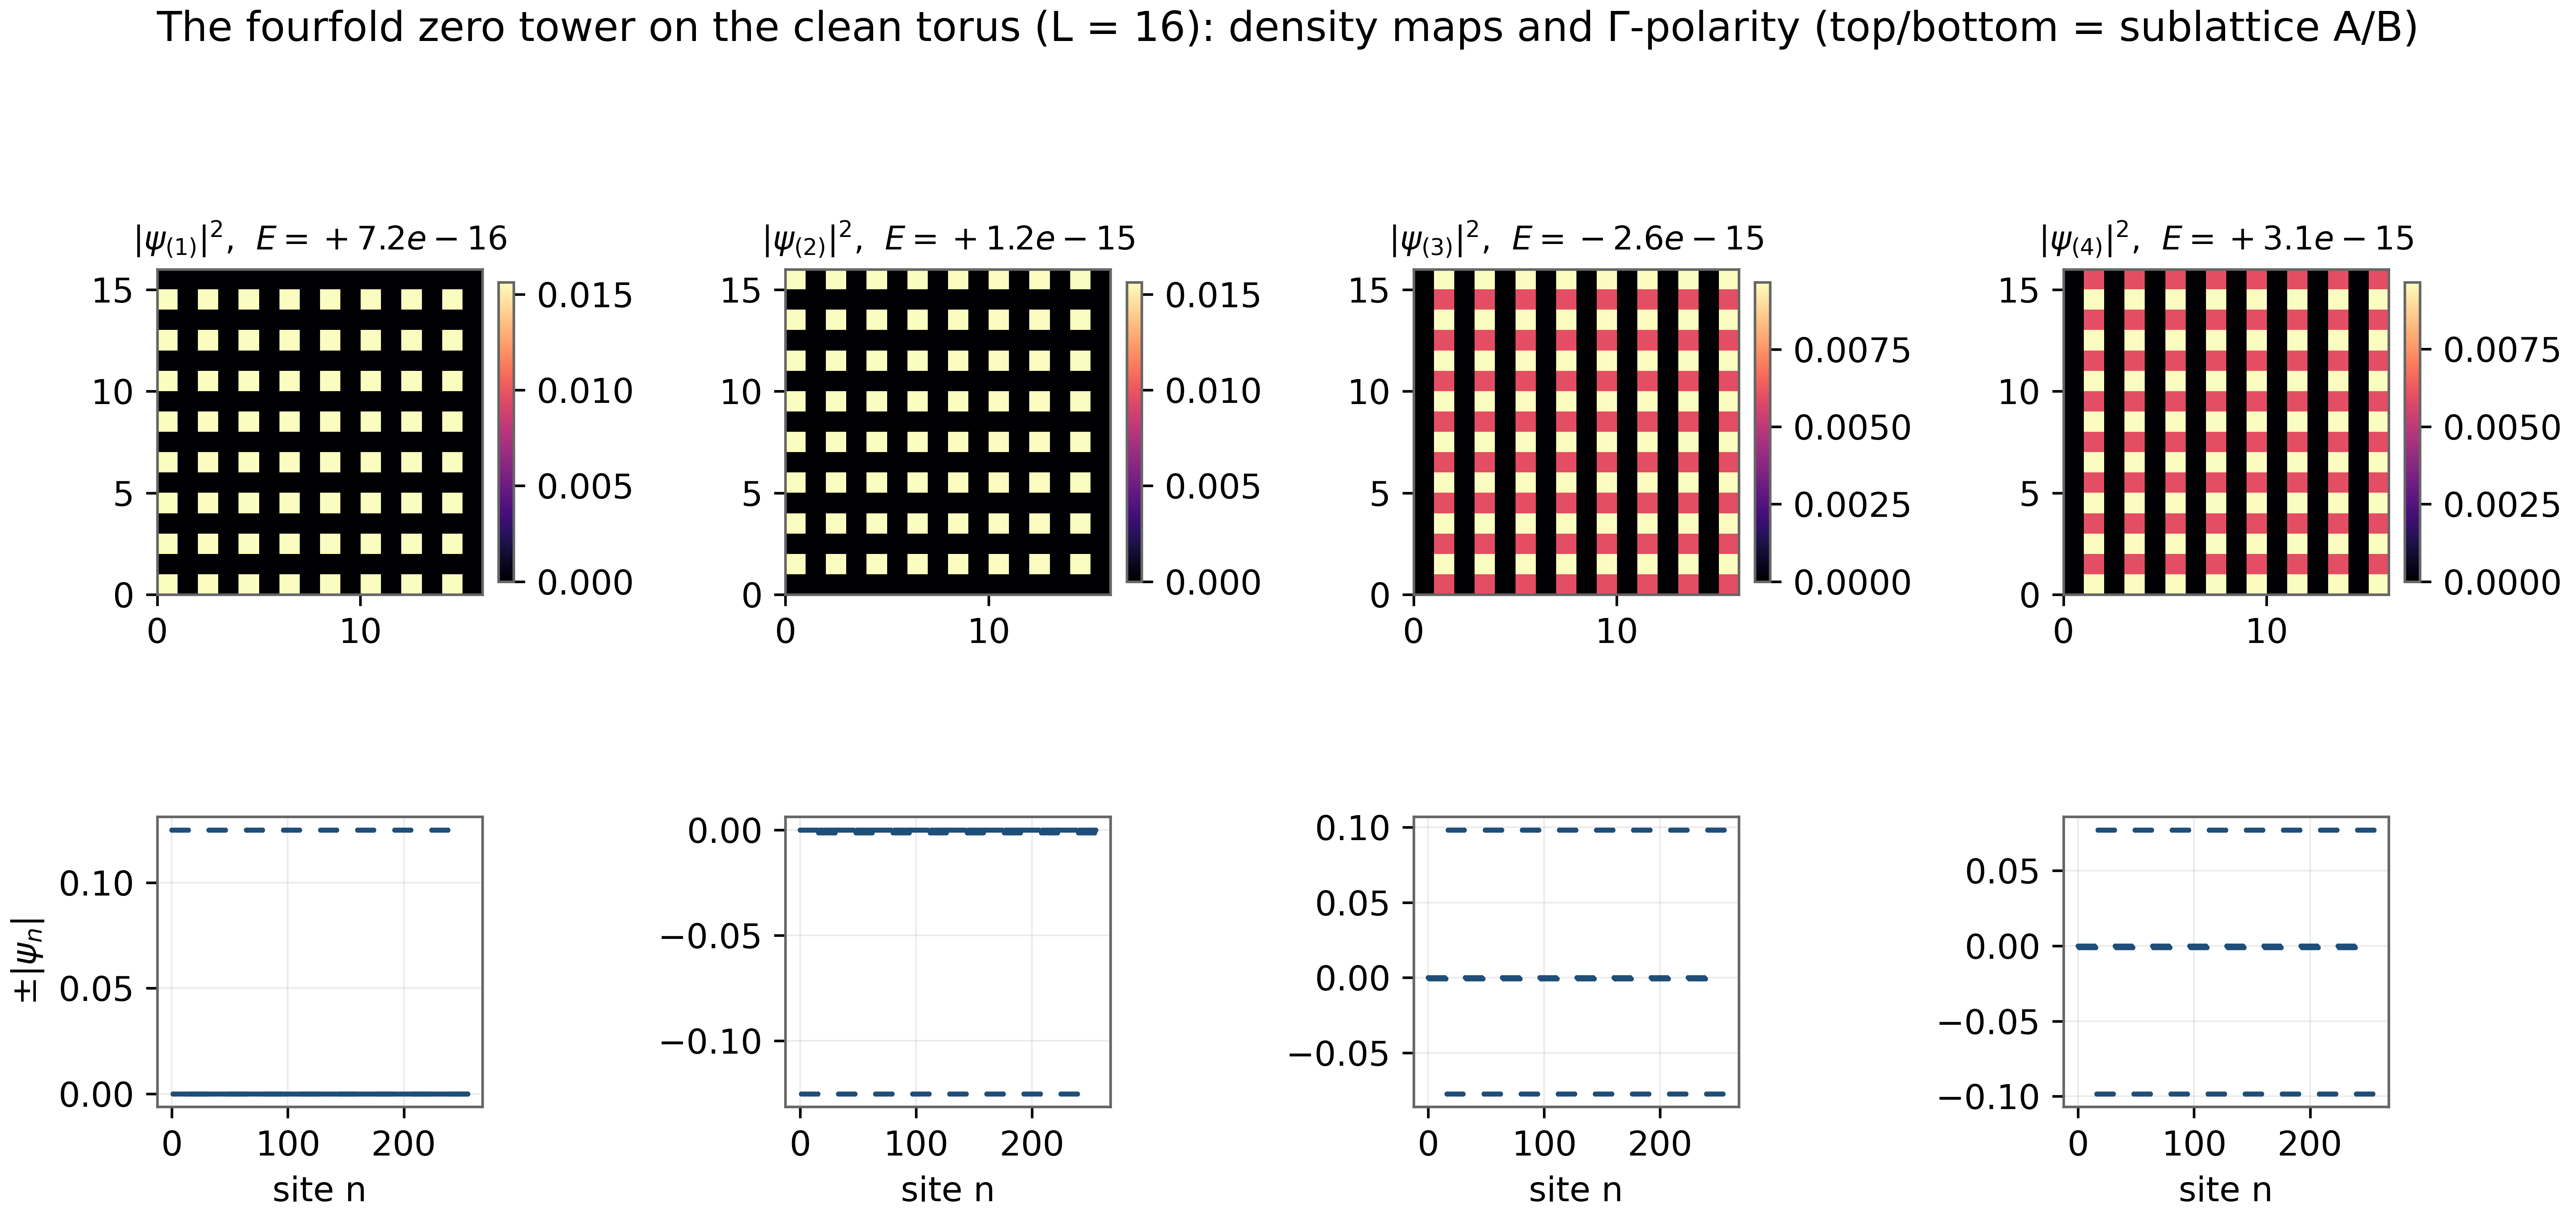
\includegraphics[max width=\columnwidth, max height=0.42\textheight]{figures/d02_extra_tower_maps.png}
\caption{Companion panels (recomputed at $L=16$): the four zero-mode densities (top) and their $\Gamma$-polarity-signed amplitudes (bottom); the two-two sublattice split is visible directly.}\label{fig:d2_2}
\end{figure}

\section{Discussion}
The tower is simultaneously the laboratory's strongest structural asset and its first honest lesson in fragility. Strongest, because a machine-precision four-fold zero subspace is exactly what the index reading of the parent suite requires. First lesson, because the same exactness makes the tower a sensitive detector: D7 will show that the $\zeta$-decoration destroys the pinning while preserving the symmetry that organized it -- an index-zero situation in the sense of Atiyah--Bott \cite{atyahbott}. The tower should therefore be read as a clean-limit signature, not as a decoration-proof invariant; D9 then shows constructively how an index-bearing decoration restores a protected subspace.

Practically, the test doubles as a health check for any modification of the substrate: if a new gauge, a new vortex layout or a new regularization breaks the tower at clean $\alpha = 1/2$, the modification has introduced same-sublattice hopping or a numerical asymmetry, and every downstream Dirac statement is in doubt. The four-line ledger of D2 is cheap insurance.

\section{Reproducibility}
\begin{itemize}[leftmargin=1.2em, itemsep=0.15em]
\item \textbf{Single test:} \texttt{python3} \path{code/dirac_lab.py} \texttt{--test D2} (add \texttt{--quick} for a reduced pass; \texttt{--no-figures} to skip the 600-dpi figure).
\item \textbf{Canonical run:} \texttt{make all} regenerates the whole D1--D14 ledger into \path{results/}; this monograph's ledger is the verbatim per-check table of that run.
\item \textbf{Determinism:} seed 96 (parent convention); the $\zeta$ tables are the Odlyzko-derived files in \path{data/} with provenance in their headers.
\item \textbf{Figures:} the canonical figure was regenerated into this folder by the v1.4 harness (the original test function itself); companion panels are recomputed with the same modules (\path{scripts/make_extra_figures.py}). All figures are 600 dpi.
\item \textbf{Cross-verification:} \texttt{julia} \path{code/dirac_lab_cross.jl} re-derives this test's verdicts from the written conventions alone (see \path{results/CROSS_VERIFICATION.md}).
\item \textbf{Artifacts in this folder:} \path{monograph.tex} (this document's source), \path{results.json} (machine-readable ledger), \path{figures/} (600-dpi figures), and the canonical CSV of the test.
\end{itemize}

\section*{References}
\begin{thebibliography}{99}\small
\bibitem{dirac} P. A. M. Dirac, The quantum theory of the electron, Proc. R. Soc. A 117, 610 (1928).
\bibitem{parent} I. K. Isaev, AB-Cloud Research: the Hofstadter--Aharonov--Bohm realization of the Hilbert--P'olya programme (parent repository and test ledger), \url{https://github.com/wild8highlander/ab-cloud-research} (2026).
\bibitem{atyahbott} M. F. Atiyah and R. Bott, The Yang--Mills equations over Riemann surfaces, Philos. Trans. R. Soc. A 308, 523 (1983).
\end{thebibliography}

\vfill
\noindent\rule{\textwidth}{0.4pt}\\[0.2em]
{\footnotesize\color{labgray} AB-Cloud Dirac Laboratory · per-test monograph series v1.4 · compiled with Tectonic (LaTeX) · all numbers traceable to \texttt{results/run\_20261006\_full\_v13} · \texttt{D2} of 14.}

\end{document}